\section{Observation and Calculations}
\subsection{Digital to Analog Conversion}
\subsubsection{3-bit input}
We constructed 3 bit R/2R ladder DAC circuit using \verb|IC741| op-amps, with a constant power supply of 5V corresponding to 1 bit and 0V corresponding to 0 bit. Fig. \ref{f1} shows the circuit in action. In Table \ref{tab:1}, we can see that observed voltage values are very close to the theoretical values calculated using Eq. \ref{eq1}. This is reflected in Fig. \ref{g1}, which shows a linear relationship between $V_\text{obs}$ and $V_\text{th}$ with a slope nearly 1 ($\approx 1.01 \pm 0.001$). All voltages obtained are negative since we use the op-amp in inverting configuration.

\begin{table}[H]
    \centering
    \begin{tabular}{|c|c|}
    \hline
     I(A)& B (Gauss) \\ \hline
     0.0 &    0 \\
     0.2 &  188 \\
     0.4 &  389 \\
     0.6 &  568 \\
     0.8 &  780 \\
     1.0 &  988 \\
     1.2 & 1170 \\
     1.4 & 1350 \\
     1.6 & 1580 \\
     1.8 & 1770 \\
     2.0 & 1980 \\
     2.2 & 2170 \\
     2.4 & 2360 \\
     2.6 & 2540 \\
     2.8 & 2740 \\
     3.0 & 2940 \\
     3.2 & 3130 \\
     3.4 & 3340 \\
     3.5 & 3420 \\
     3.6 & 3500 \\
     3.7 & 3600 \\
     3.8 & 3690 \\
     3.9 & 3790 \\
     4.0 & 3870 \\
    \hline
    \end{tabular}
    \caption{Data for calibration}
    \label{tab:1}
\end{table}

\begin{figure}
    \centering
    \includegraphics[width=1\columnwidth]{images/3bit.eps}
    \caption{$V_\text{obs}$ vs. $V_\text{th}$ for a 3-bit DAC}
    \label{g1}
\end{figure}

\subsubsection{4-bit input}
Similarly, we constructed a 4-bit DAC (by adding an additional $R-2R$ ladder in Fig. \ref{obj:1}). In Table \ref{tab:1.5}, we can see that observed voltage values are very close to the theoretical values calculated using Eq. \ref{eq2}. Fig. \ref{graph:2} again shows a linear relationship between $V_\text{obs}$ and $V_\text{th}$ with a slope nearly 1 ($\approx 0.99 \pm 0.0009$).

\begin{table}[H]
    \centering
    \begin{tabular}{|c|c|c|c|c|c|c|c|}
        \hline
        bit-0 (MSB) & bit-1 & bit-2 & bit-3 (LSB) & $V_\text{obs}$ (V)& $ V_\text{th}$ (V) \\ \hline
0 & 0           & 0     & 0           & 0      & 0\\ \hline
0 & 0           & 0     & 1           & -0.635        & -0.636\\ \hline
0 & 0           & 1     & 0           & -1.287        & -1.272 \\ \hline
0 & 0           & 1     & 1           & -1.914        & -1.908\\ \hline
0 & 1           & 0     & 0           & -2.563        & -2.545\\ \hline
0 & 1           & 0     & 1           & -3.199         & -3.181\\ \hline
0 & 1           & 1     & 0           & -3.84        & -3.82\\ \hline
0 & 1           & 1     & 1           & -4.47         & -4.45\\ \hline

1& 0           & 0     & 0           & -5.09 & 5.09\\ \hline
1& 0           & 0     & 1           & -5.71        & -5.73\\ \hline
1& 0           & 1     & 0           & -6.37        & -6.36\\ \hline
1& 0           & 1     & 1           & -6.99        & -6.99\\ \hline
1& 1           & 0     & 0           & -7.64         & -7.63\\ \hline
1& 1           & 0     & 1           & -8.27         & -8.27\\ \hline
1& 1           & 1     & 0           & -8.91         & -8.91\\ \hline
1& 1           & 1     & 1           & -9.54         & -9.54\\ \hline
    \end{tabular}
    \caption{Output of 4 bit DAC using $R=1$ k$\ohm$ resistors}
    \label{tab:1.5}
\end{table}

\begin{figure}
    \centering
    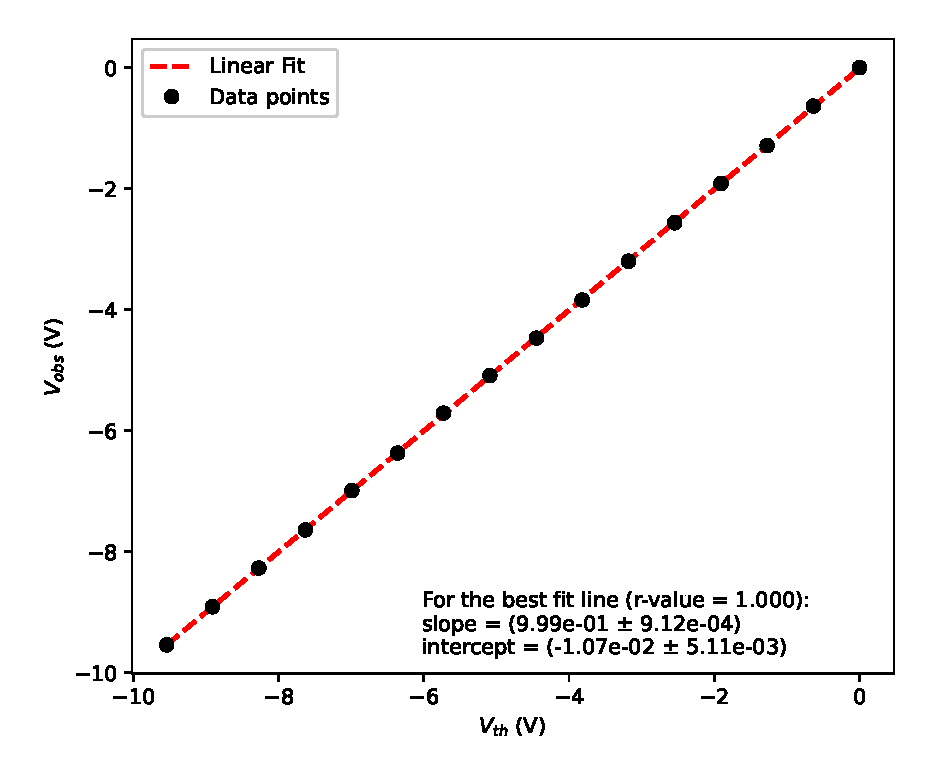
\includegraphics[width=1\columnwidth]{images/4bit.eps}
    \caption{$V_\text{obs}$ vs. $V_\text{th}$ for a 4-bit DAC}
    \label{graph:2}
\end{figure}

For both the circuits we can see a very small deviation in the observed values from the theoretical values. This could be because we have assumed $R=1$ k$\Omega$ in all our calculations. The actual value of $R$ can vary since the resistors we used were a combination of 1\% and 20\% tolerance resistors.


\subsection{Analog to Digital Converter}
% \subsubsection{Working of comparator}
We used three out of four comparators available in \verb|LM339| and verified it's working for a 5V constant power supply.
Now, using \verb|LM339| comparator and \verb|74147| priority encoder, we constructed the 2-bit digital to the analog circuit using the circuit in Figure \ref{obj:2}. Finally to convert binary to human decimal outputs, we used \verb|IC 7447| (binary to BCD decoder) chip which then connected to a common anode BCD display via a 330 k$\Omega$ resistors.

From Table \ref{tab:3}, we can verify it's working. It succesfully converts analog signal into 2-bit digital output. Fig. \ref{f2} shows all of the combination of input and output values achived based on Table \ref{tab:3}.

\begin{table}[H]
    \centering
    \begin{tabular}{|c|c|c|c|c|c|}
        \hline
        Fringe    & Fringes on     & Fringes on       & $\text{D}_x$        & $\rho_x$   & $\text{R}_x$    \\ 
        Order     & the left (mm)  & the right (mm)   & (mm)       & ($\text{mm}^2$)   & (mm)   \\ \hline
        1 &  9.24 & 5.40 &  3.84 &     &     \\
         2 & 10.38 & 3.89 &  6.49 &  6.84 & 11.62 \\
         3 & 11.18 & 3.02 &  8.16 & 12.96 & 11.00  \\
         4 & 12.41 & 2.23 & 10.18 & 22.22 & 12.58 \\
         5 & 13.05 & 1.48 & 11.57 & 29.78 & 12.64 \\
         6 & 13.55 & 0.82 & 12.73 & 36.83 & 12.50 \\
         7 & 14.10 & 0.18 & 13.92 & 44.76 & 12.66 \\\hline
       \end{tabular}
    \caption{Observed fringe pattern on along the longitudinal direction}
    \label{tab:3}
\end{table}

% \begin{figure}[H]
%     \centering
%     \includegraphics[width=1\columnwidth]{images/2.jpg}
%     \caption{ADC circuit constructed on a breadboard. The output shown here on the BCD is 2 V. The lower LEDs show that 2 comparators are active. The above LED's show the ADC output in binary (10) which again corresponds to 2 V.}
%     \label{f2}
% \end{figure}


\begin{figure}[H]
    \centering
    \includegraphics[width=1\columnwidth]{images/dac.jpg}
    \caption{3-bit DAC circuit constructed on a breadboard. The input (shown using the LEDs) is $011$ corresponding to -3.83 V on the multimeter (not pictured here).}
    \label{f1}
\end{figure}

\begin{figure}[H]
    % \ContinuedFloat
    % \bigskip
    \begin{subfigure}{\linewidth}
    \includegraphics[width=1\textwidth]{images/0.jpg}
    \caption{Analog output 0}
    \end{subfigure}
    
    % % \bigskip
    % \begin{subfigure}{\linewidth}
    % \includegraphics[width=1\textwidth]{images/1.jpg}
    % \caption{}
    % \end{subfigure}

    % \begin{subfigure}{\linewidth}
    % \includegraphics[width=1\textwidth]{images/2.jpg}
    % \caption{}
    % \end{subfigure}
    
    % \begin{subfigure}{\linewidth}
    % \includegraphics[width=1\textwidth]{images/3.jpg}
    % \caption{}
    % \end{subfigure}
            
    % \caption{ADC circuit constructed on a breadboard, along with the BCD analog output. The 2 LEDs on the top represent the (inverted) IC 74147 output and the 3 LEDs below show represent the comparator output. }
    % \label{f2}
\end{figure}


\begin{figure}[H]
    \ContinuedFloat
    % \bigskip
    % \begin{subfigure}{\linewidth}
    % \includegraphics[width=1\textwidth]{images/0.jpg}
    % \caption{Analog output 0}
    % \end{subfigure}
    
    \begin{subfigure}{\linewidth}
        \includegraphics[width=1\textwidth]{images/1.jpg}
        \caption{Analog output 1}
    \end{subfigure}
    
    \bigskip
    \begin{subfigure}{\linewidth}
        \includegraphics[width=1\textwidth]{images/2.jpg}
        \caption{Analog output 2}
    \end{subfigure}
    
    \bigskip
    \begin{subfigure}{\linewidth}
    \includegraphics[width=1\textwidth]{images/3.jpg}
    \caption{Analog output 3}
    \end{subfigure}
            
    \caption{ADC circuit constructed on a breadboard, along with the BCD analog output. The 2 LEDs on the top represent the (inverted) IC 74147 output and the 3 LEDs below show represent the comparator output. }
    \label{f2}
\end{figure}